%======================================================
% Technische Universitaet Darmstadt
% Fachbereich Elektrotechnik und Informationstechnik
% Fachbereich Informatik (Zweitmitglied)
% Fachgebiet Multimedia Kommunikation (KOM)
% Prof. Dr.-Ing. Ralf Steinmetz
%======================================================
% Template for Theses
% VERSION 1.3 (November 2017)
% Use pdfLaTeX (other possible, but not supported)
% Contact at KOM: Andr\'e Miede (andre.miede@kom...)
%======================================================
% Official TUD-LaTeX-files have to be installed:
% http://exp1.fkp.physik.tu-darmstadt.de/tuddesign/
% Refer to the manuals and forum for details
%======================================================
\documentclass[longdoc,accentcolor=tud1b,11pt,paper=a4]{tudreport}
%======================================================
% colorback = Bereich unter Titel mit Hintergrundfarbe
% colorbacktitle = Titel mit Hintergrundfarbe (Akzent)
% KOM-Blau = accentcolor=tud1b		
% Grau = accentcolor=tud0a 
% blackrule fuer schwarze Leiste
% nochapterpage = do not start chapters on new page
% oneside = print only on one side of the page
%======================================================

%======================================================
% General package loading and definitions
%======================================================
\usepackage[utf8]{inputenc}
\usepackage{textcomp} 
% \usepackage{ngerman}
\usepackage[american,ngerman]{babel}
\usepackage{xspace}
\usepackage[fleqn]{amsmath} % math environments and more by the AMS 
\newcounter{dummy} % necessary for correct hyperlinks (to index, bib, etc.)
\newcommand{\myfloatalign}{\centering} % how all the floats will be aligned

%======================================================
% packages added by the author
%======================================================
\usepackage{float}
\usepackage{wrapfig}
\usepackage[toc, page]{appendix}

%======================================================
% KOM-modifications of the TUD-layout
%======================================================
% reduce font size of page footers and headers (fancyhdr)
\renewcommand{\footerfont}{\fontfamily{\sfdefault}\fontseries{m}\fontshape{n}\footnotesize\selectfont}
% remove space between items 
\usepackage{enumitem}
	\setenumerate{noitemsep}
	\setitemize{noitemsep}
	\setdescription{noitemsep}
%\setlist{nolistsep}

%======================================================
% Package loading for example contents (content.tex)
%======================================================
\usepackage{verbatim}
\usepackage{tabularx} % better tables
\setlength{\extrarowheight}{3pt} % increase table row height
\usepackage{booktabs}
\usepackage{caption}
\captionsetup{format=hang,font=small}
\usepackage[square,numbers]{natbib}
\usepackage{subfig}
\usepackage[stable,bottom]{footmisc}
\usepackage{framed}
\usepackage{color}

%======================================================
% Flags
%======================================================
\newboolean{final} %Deklaration
\setboolean{final}{false} %Zuweisung


%======================================================
% Important information: to be set here and only here
%======================================================

% Title of the thesis in DE or EN, depending on thesis language
\newcommand{\komTitle}{Application of the Lottery Ticket Hypothesis in NLP and Early Pruning (Proposal)\xspace} 
% Translation of the title in either DE or EN, depending on thesis language
\newcommand{\komTitleTranslation}{Anwendung der "Lottery Ticket"-Hypothese in NLP und frühem Pruning (Proposal)\xspace}

% Typ der Arbeit: Diplomarbeit Studienarbeit Master-Arbeit Bachelor-Arbeit
\newcommand{\komThesisType}{Bachelor-Arbeit\xspace} 

% Studiengang: Elektrotechnik und Informationstechnik, Informationssystemtechnik, Informatik, ...
\newcommand{\komCourseOfStudy}{Computational Engineering\xspace}

\newcommand{\komName}{Tim Unverzagt\xspace}
\newcommand{\komSubmissionDate}{dd. month yyyy\xspace}% use only this date format

\newcommand{\komGutachter}{Gutachter: ???\xspace}
\newcommand{\komBetreuer}{Betreuerin: Anna Filighera\xspace}
\newcommand{\komExternerBetreuer}{}
\newcommand{\komID}{KOM-type-number ???\xspace}



%======================================================
% Setup for hyperref
%======================================================
\usepackage[pdftex,hyperfootnotes=true,pdfpagelabels]{hyperref}
	\pdfcompresslevel=9
	\pdfadjustspacing=1 
\hypersetup{%
    colorlinks=false, linktocpage=false, pdfstartpage=1, pdfstartview=FitV,%
    breaklinks=true, pdfpagemode=UseNone, pageanchor=true, pdfpagemode=UseOutlines,%
    plainpages=false, bookmarksnumbered, bookmarksopen=true, bookmarksopenlevel=1,%
    hypertexnames=true, pdfhighlight=/O, %nesting=true,%frenchlinks,%
    %urlcolor=tud1b, linkcolor=tud1b, citecolor=tudtud1bccent,
    pdftitle={\komTitle, \komThesisType, \komID},%
    pdfauthor={\komName, KOM, TU Darmstadt},%
    pdfsubject={},%
    pdfkeywords={},%
    pdfcreator={},%
    pdfproducer={}%
}

%============================================
% Setup of the title page (do not change)
%============================================

\title{\komTitle}
\subtitle{\komTitleTranslation \\ \komThesisType}
\subsubtitle{\komName \\ \komID}
%\setinstitutionlogo[height]{kom_info}
\institution{\raggedleft Fachbereich Informatik\\%
	Fachbereich ??? (Zweitmitglied)\\[\baselineskip]%
	Fachgebiet Natural Language Processing \\%(KOM)
	|Gutachter|}

%============================================
% Setup of the title backside (do not change)
%============================================
\lowertitleback{%
	Technische Universität Darmstadt \\%
	Fachbereich Informatik\\%
	Fachbereich ??? (Zweitmitglied)\\[\baselineskip]%
	Fachgebiet Natural Language Processing (KOM)\\%
	|Gutachter|%
	%Department of Electrical Engineering and Information Technology \\%
	%Department of Computer Science (Adjunct Professor) \\[\baselineskip]%
	%Multimedia Communications Lab (KOM) \\%
	%Prof. Dr.-Ing. Ralf Steinmetz %
}


\uppertitleback{%
    \textbf{\komTitle} \\%
    \komTitleTranslation \\[\baselineskip]%
	\komThesisType \\%
    Studiengang: \komCourseOfStudy \\%
	\komID \\[\baselineskip]%
	Eingereicht von \komName \\%
	Tag der Einreichung: \komSubmissionDate \\[\baselineskip]%
	\komGutachter \\%
	\komBetreuer \\%
	\komExternerBetreuer%
}
	
%======================================================
% MAIN DOCUMENT STARTS HERE
%======================================================
\begin{document}
	
	\colorlet{tudidentbar}{tud1b} %first page colored - DO NOT MODIFY THIS
	%======================================================
	% The front matter
	%======================================================
	\pagenumbering{roman}
	\frenchspacing
	\raggedbottom
	\selectlanguage{american} % american ngerman
	\maketitle
	
	% identbar color for the rest of the thesis - DO NOT MODIFY THIS
	\colorlet{tudidentbar}{tud0b} 

    \begin{otherlanguage}{ngerman}
    \chapter*{Erklärung zur Abschlussarbeit gemäß § 23 Abs.\ 7 APB der TU Darmstadt}
    Hiermit versichere ich, \komName, die vorliegende \komThesisType ohne Hilfe Dritter und nur mit den angegebenen Quellen und Hilfsmitteln angefertigt zu haben. 
    Alle Stellen, die Quellen entnommen wurden, sind als solche kenntlich gemacht worden. 
    Diese Arbeit hat in gleicher oder ähnlicher Form noch keiner Prüfungsbehörde vorgelegen.\\

    \noindent Mir ist bekannt, dass im Falle eines Plagiats (§38 Abs.2 APB) ein Täuschungsversuch vorliegt, der dazu führt, dass die Arbeit mit 5,0 bewertet und damit ein Prüfungsversuch verbraucht wird. 
    Abschlussarbeiten dürfen nur einmal wiederholt werden.\\

    \noindent Bei der abgegebenen \komThesisType stimmen die schriftliche und die zur Archivierung eingereichte elektronische Fassung überein. 
    
    \vspace{4em}
    
    \noindent Darmstadt, den \komSubmissionDate 
    
    \vspace{3em}
    
    \noindent\rule{5cm}{0.4pt}
    
    \noindent\komName
    
    \end{otherlanguage}
    

    % Old Version (do not use if submitting via the TUBaMa-Portal!)
    %\chapter*{Ehrenw\"ortliche Erkl\"arung}
    %Hiermit versichere ich, die vorliegende \komThesisType ohne Hilfe Dritter und nur mit den angegebenen Quellen
    %und Hilfsmitteln angefertigt zu haben. Alle Stellen, die aus den Quellen entnommen wurden, sind als solche
    %kenntlich gemacht worden. Diese Arbeit hat in dieser oder \"ahnlicher Form noch keiner Pr\"ufungsbeh\"orde vorgelegen.
    %Die schriftliche Fassung stimmt mit der elektronischen Fassung \"uberein.
    %
    %\vspace{1.5cm}
    %
    %\noindent Darmstadt, den \komSubmissionDate\hfill \komName

	
	\tableofcontents
	%\listoffigures
	%\listoftables
	
	%======================================================
	% The main matter (insert your contents here)
	%======================================================
	\cleardoublepage
	\pagenumbering{arabic}
	
\newcommand{\hint}[1]{
  \ifthenelse{\boolean{final}}{}{
\textcolor{green}{   
	\begin{framed}
	\noindent
	\underline{Hint:}\\ \newline
	#1
	\end{framed}
}
}}
	\begin{abstract}
 The abstract goes here...
\end{abstract}




%*****************************************
\chapter{Introduction}
%*****************************************
\hint{This chapter should motivate the thesis, provide a clear description of the problem to be solved, and describe the major contributions of this thesis. The chapter should have a length of about two pages!}

\section{Motivation}
What is the motivation for doing research in this area?

\section{Problem Statement and Contribution}
What is the problem that should be solved with this thesis?

\section{Outline}
How is the rest of this thesis structured?



%*****************************************
\chapter{Background}
\label{ch:background}
%*****************************************
\hint{This chapter should give a comprehensive overview on the background necessary to understand the thesis.
The chapter should have a length of about five pages!}


\section{Basics of Neural Networks\ \ \  \(WIP\)}
Neural networks are a part of most major AI-breakthrough in the last decade enabling computers to compete in fields formerly championed by humans.\footnote[1]{
	\begin{itemize}
		\item 
			2011: "Watson" of IBM defeats two former grand champions in "Jeopardy!" \cite{lally2011natural}
		\item 
			2011: "Siri" enables users to use natural language to interact with their phones 
			\cite{ARON201124}
		\item 
			2015: A convolutional neural network classifies images from the ImageNet dataset more accurately than human experts 
			\cite{Russakovsky2015} \cite{He_2015_ICCV}
		\item 
			2016: "AlphaGo" beats Lee Sedol, one of the world's strongest Go players
			\cite{gibney2016google} \cite{silver2017mastering}
	\end{itemize}
}
They implement a statistical understanding of AI, which is to say that they try to find a specific model optimizing the likelihood of reproducing input-output pairs similar to some training data. The competing philosophy directly divines behaviour rules, frequently from expert knowledge, and as such is far less dependant from data.  
\textcolor{red}{[citation needed]}\\
For the former concept its model classes are the essential point of design. A multitude of properties are sought after in a model class of which a few are:
\begin{itemize}
	\item Richness: The diversity of single models in the class and thus the ability to fit a wide field of different input-output landscapes
	\item Stability of models: Tendency of any model in the class to not produce sudden unmotivated change in behaviour between and beyond given data points
	\item Interpretability of models: Ease of formulating knowledge out of any given model in the class.
	\item ...
	\item \textcolor{red}{[citation needed]}
\end{itemize}
If one knows an agent that already performs well on a given task it is sensible to design ones model class to reproduce its decision process. As Humans embody such an agent for many tasks of interest to AI research naturally their processing system e.g. their central nervous system is the direct inspiration for neural networks approaches.\\
The human central nervous system is, in all simplicity, a network of neurons which can receive multiple stimuli and are able to produce an output if stimulated to a certain degree. The stimuli received by neurons are either from an external source or another neuron's output.
\textcolor{red}{[citation needed]}
One such neuron and its stimulus measure are depicted in Figure \ref{fig:neuron1}. Another detail of design observed in nature is the ability of a neuron to vary the strength of connection to any source of stimulus. 
\textcolor{red}{[citation needed]}\\
In addition to variable weights of inputs and an activation function, the abstract neuron
seen in Figure \ref{fig:neuron2} also allows for a variable base stimulus generally called "bias". It thus completes a canonical neuron which forms the basis unit for neural networks.\\


\begin{figure}
	\centering
	\begin{minipage}{0.45\textwidth}
		\centering
		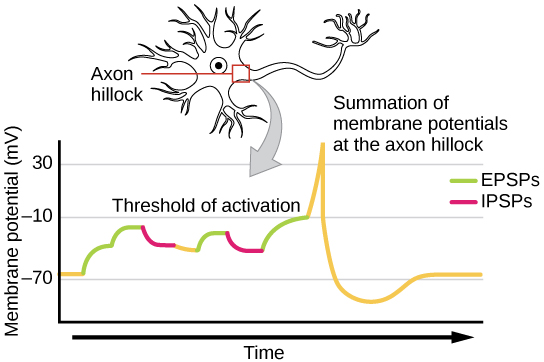
\includegraphics[height=150px]{gfx/Biological_Neuron.jpg}
		\caption{Representation of a biological Neuron}
		\label{fig:neuron1}
	\end{minipage}\hfill
	\begin{minipage}{0.45\textwidth}
		\centering
		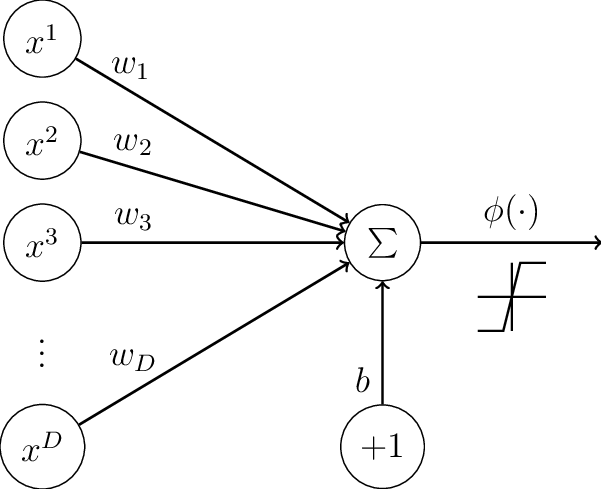
\includegraphics[height=150px]{gfx/Abstract_Neuron.png}
		\caption{Abstraction of a Neuron}
		\label{fig:neuron2}
	\end{minipage}
\end{figure}

As the individual neurons is too simple to model any complex relation between inputs
and outputs the next step is to aggregate multiple neurons. Figure \ref{fig:FFNetwork} displays a few neurons coming together to form a simple fully-connected feed-forward network.
\footnote[2]{
	Inputs of neural networks are often called "features" and fully-connected networks are frequently referred to as "dense"	}
\begin{figure}
	\centering
		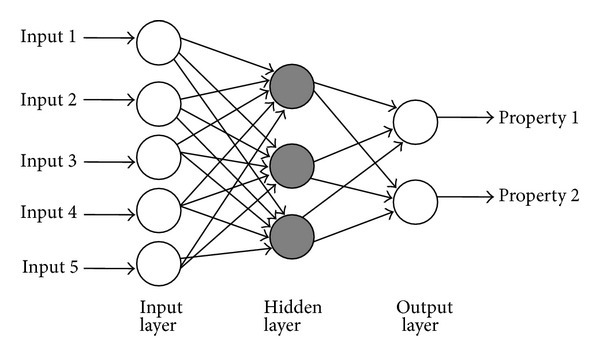
\includegraphics[height=150px]{gfx/Dense_FFNetwork.jpg}
		\caption{A small fully-connected network}
		\label{fig:FFNetwork}
\end{figure}

\begin{itemize}
	\item \textcolor{red}{TODO:}
	\item Issue of computational expense
	\item CNNs (and other forms of NN?)
\end{itemize}
	
\section{The Lottery Ticket Hypothesis}
\begin{itemize}
	\item \textcolor{red}{TODO:}
	\item Clarifying the task (image classification)
	\item Issue of overloading on parameters
	\item Idea of trainable subnets
	\item Emergence of safe "return points" after a few training epochs
	\item (?) Ablation study
\end{itemize}

\section{Basics of Natural Language Processing}
\begin{itemize}
	\item \textcolor{red}{TODO:}
	\item (?) Corpora
	\item Tokenizing
	\item Language Models
\end{itemize}

\section{Combining LMs \& CNNs}
\begin{itemize}
	\item \textcolor{red}{TODO:}
	\item Interpreting the tensor representation of a sentence/document as an image to be classified
	\item (?) Validation through results
	\item (?) Handeling different sizes of inputs
	\item (?) Handeling missing words in the Language model
\end{itemize}


%*****************************************
\chapter{Related Work}
\label{ch:relatedwork}
%*****************************************
\hint{This chapter should give a comprehensive overview on the related work done by other authors followed by an analysis why the existing related work is not capable of solving the problem described in the introduction.
The chapter should have a length of about three to five pages!}
\section{Related Work Dynamic Pruning}

\section{Related Work Network Architecture Search}

\section{Analysis of Related Work}

\section{Summary}

%*****************************************
\chapter{Design}
\label{ch:design}
%*****************************************
\hint{This chapter should describe the design of the own approach on a conceptional level without mentioning the implementation details. The section should have a length of about five pages.}

\section{Requirements and Assumptions}

\section{System Overview}

\subsection{Component 1}

\subsection{Component 2}

\section{Summary}

%*****************************************
\chapter{Implementation}
\label{ch:implementation}
%*****************************************

\hint{This chapter should describe the details of the implementation addressing the following questions: \\ \\
1. What are the design decisions made? \\
2. What is the environment the approach is developed in? \\
3. How are components mapped to classes of the source code? \\
4. How do the components interact with each other?  \\
5. What are limitations of the implementation? \\ \\
The section should have a length of about five pages.}
\section{Design Decisions}

\section{Architecture}

\section{Interaction of Components}

\section{Summary}

%*****************************************
\chapter{Evaluation}
\label{ch:evaluation}
%*****************************************
\hint{This chapter should describe how the evaluation of the implemented mechanism was done. \\ \\
1. Which evaluation method is used and why? Simulations, prototype? \\
2. What is the goal of the evaluation? Comparison? Proof of concept? \\
3. Wich metrics are used for characterizing the performance, costs, fairness, and efficiency of the system?\\
4. What are the parameter settings used in the evaluation and why? If possible always justify why a certain threshold has been chose for a particular parameter.  \\
5. What is the outcome of the evaluation? \\ \\
The section should have a length of about five to ten pages.}
\section{Goal and Methodology}

\section{Evaluation Setup}

\section{Evaluation Results}

\section{Analysis of Results}


%*****************************************
\chapter{Conclusions}
\label{ch:closure}
%*****************************************

\hint{This chapter should summarize the thesis and describe the main contributions of the thesis. Subsequently, it should describe possible future work in the context of the thesis. What are limitations of the developed solutions? Which things can be improved?
The section should have a length of about three pages.}

\section{Summary}

\section{Contributions}

\section{Future Work}

\section{Final Remarks}

	
	%======================================================
	% The back matter
	%======================================================
	%\cleardoublepage
	\refstepcounter{dummy}
	\addcontentsline{toc}{chapter}{\bibname}
	\bibliographystyle{alpha} % <--- layout of the bib
	\bibliography{bibliography,gfx/images} % file name of your bib
	
	
	%======================================================
	% Appendix (not present in the template)
	%======================================================
	\begin{appendices}

%\chapter{A history of neural networks}
%\begin{itemize}
%	\item 1. wave: ~ 1955-1970
%	\item 2. wave: ~ 1985-2000 \(?\)
%	\item 3. wave: ~ ??? 
%\end{itemize}
%\begin{figure}
%	\centering
%	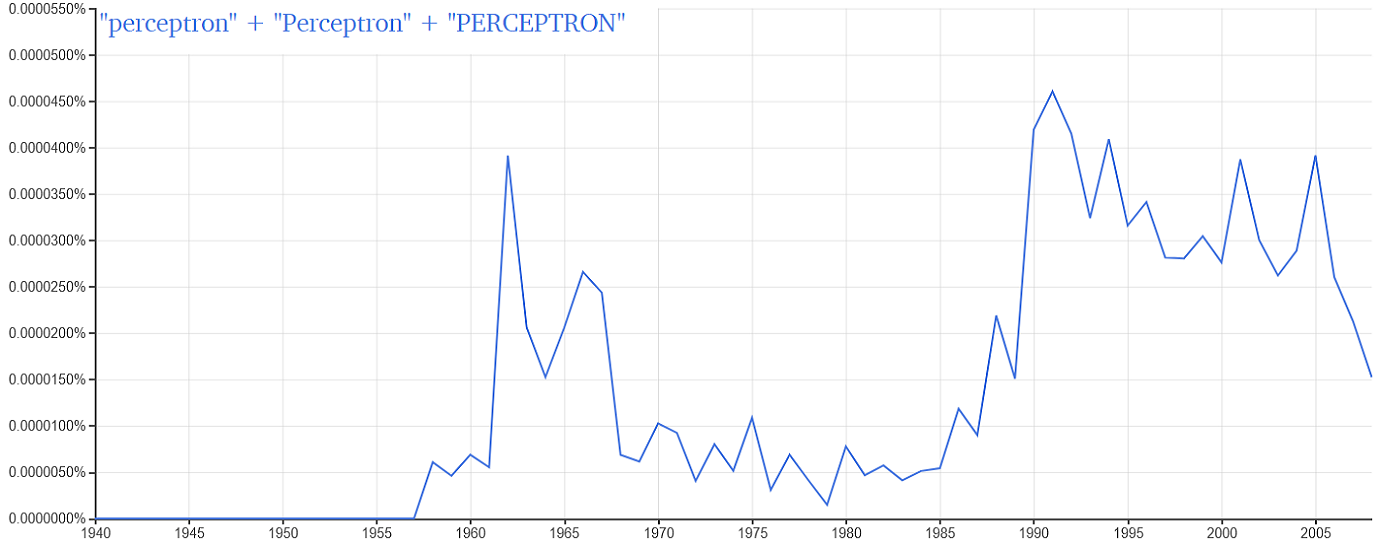
\includegraphics[height=150px]{gfx/NGrams_Perceptron.png}
%	\caption{Relative amount of occurences of the word "Perceptron" in published books between 1940 and 2009}
%\end{figure}
%\begin{figure}
%	\centering
%	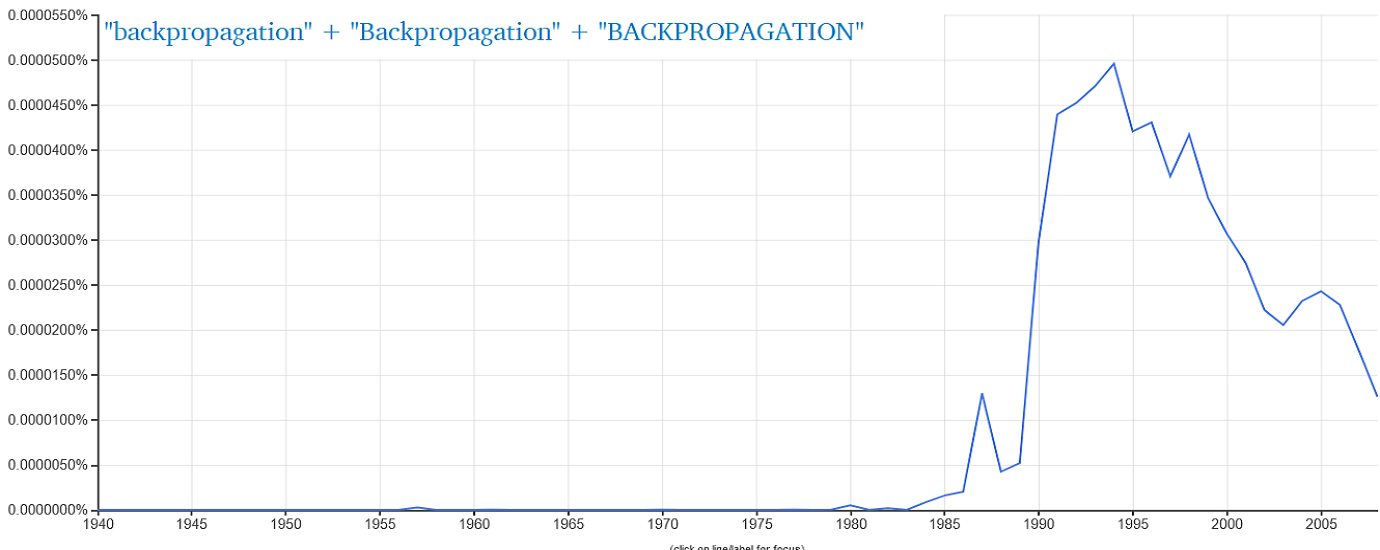
\includegraphics[height=150px]{gfx/NGrams_Backpropagation.png}
%	\caption{Relative amount of occurences of the word "Backpropagation" in published books between 1940 and 2009}
%	\label{fig:NGBackprop}
%\end{figure}

\end{appendices}

\end{document}
%======================================================
%======================================================
